\section*{Results}

\begin{figure}[ht]
\centering
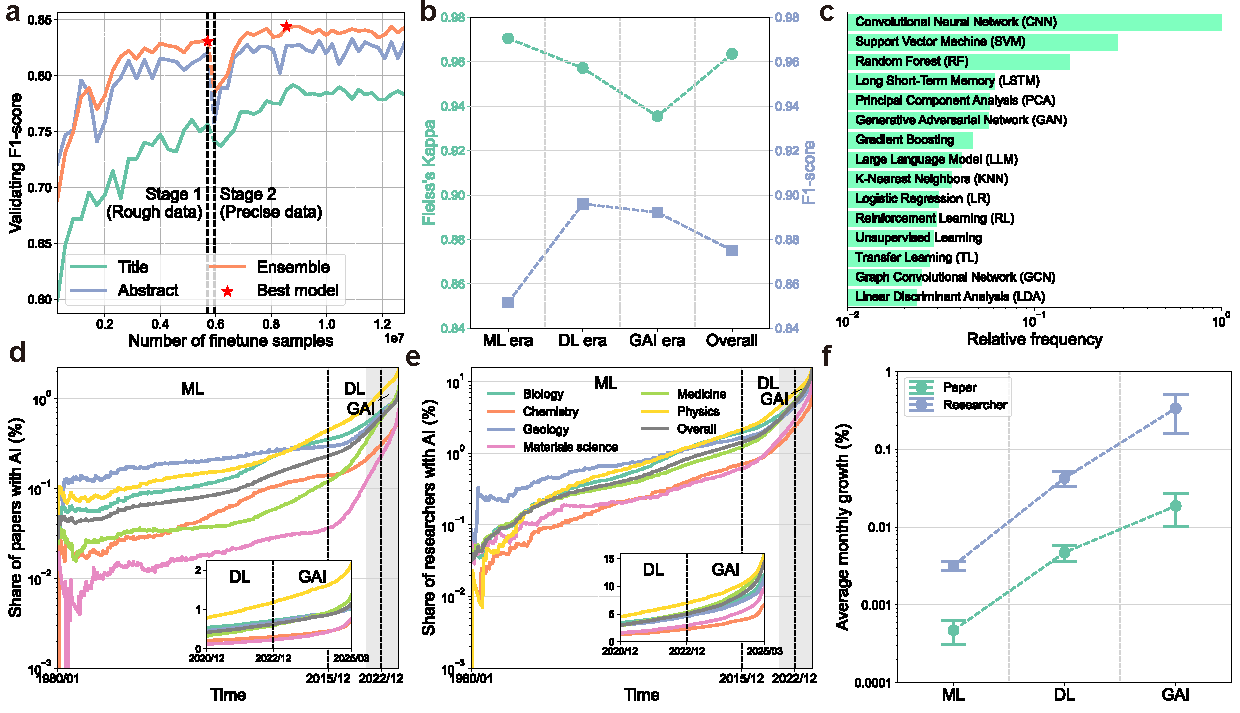
\includegraphics[width=\textwidth]{figure/1.pdf}
\caption{
\textbf{Increasing prevalence of AI adoption in science.}
\textbf{(a)} Increasing performance of AI paper identification during the two-stage fine-tuning of the BERT pre-trained models, where we use rough training data in Stage 1 to evolve precise assessments in Stage 2.
We independently train two models based on titles and abstracts, respectively, and then integrate them into an ensemble that selects the optimal models during both stages (red stars) to identify all selected papers.
\textbf{(b)} Accuracy evaluation of our identification results by human experts.
For samples spanning three eras of AI, experts reached consensus with Fleiss’ Kappa ($\kappa$) $\geq 0.93$.
Our model identification results have strong accuracy in validation against expert-labeled data with an F1-score $\geq 0.85$.
\textbf{(c)} Relative adoption frequency of the top 15 AI methods across all disciplines for all selected AI development eras.
\textbf{(d)-(e)} The growth of AI-augmented papers (d, $n=41,298,433$) and AI-adopted researchers (e, $n=5,377,346$) across the eras of ML, DL, and GAI between 1980 and 2025 in selected scientific disciplines. The y-axes are set to log-scale.
\textbf{(f)} The average monthly growth rates for AI papers and researchers across the eras of ML, DL, and GAI across all selected disciplines ($n=543$ month observations), where 99\% CIs are shown as error bars centred at the mean.
}
\label{fig1}
\end{figure}


\subsection*{Increasing prevalence of AI in science}
In this investigation, we focus on research papers using AI methods in various fields of natural science, where we conduct our analysis based on 41,298,433 papers from the OpenAlex dataset~\supercite{openalex}, covering six representative disciplines: biology, chemistry, geology, materials science, medicine, and physics (Methods~M1).
According to the invention of milestone technologies in the trend of AI development, we divide the past decades into three eras, namely machine learning (ML), deep learning (DL), and generative AI (GAI) (Methods~M2).
To identify AI papers in various fields across eras, we fine-tune BERT~\supercite{DBLP:conf/naacl/DevlinCLT19,wolf-etal-2020-transformers}, an established language model~\supercite{DBLP:conf/emnlp/BeltagyLC19,DBLP:conf/acl/CohanFBDW20,DBLP:conf/emnlp/SinghDCDF23}, on articles published in explicitly AI-oriented scientific journals and conferences for automatically extracting and interpreting information from context.
Specifically, we employ a two-stage fine-tuning process to adapt the pre-trained BERT model to the task of AI paper identification.
We first independently train two models based on titles and abstracts of papers, respectively, then ensemble the optimized individual models to identify all selected papers (Fig. 1a, Methods~M3, and Extended Data Fig. 1).
This approach eliminates the need for manual selection of AI-related trigger words, as demonstrated in previous research~\supercite{frank2019evolution}.

To evaluate the accuracy of our identification, we recruited a team of human experts to validate these results (Methods~M4 and Extended Data Fig. 2).
The experts demonstrate strong consensus across their independent annotation of papers sampled at random from the six disciplines mentioned above, achieving an average Fleiss’ Kappa ($\kappa$) of 0.964~\supercite{landis1977measurement,fleiss1971measuring}. The BERT model attains an F1-score of 0.875 in an evaluation that uses the expert labels as ground truth.
Meanwhile, the strong consensus among experts and high quality for identification is consistent across samples from different eras of AI, confirming the reliability of our identification accuracy and laying a robust foundation for our subsequent analysis (Fig. 1b and Supplementary Table~S1-S4).
To provide a rationale and explainability for our identification results, we visualize attention strengths in the BERT model with examples, where the model allocates substantial attention to terms such as “neural network” and “large language model”, illustrating how the model correctly interprets and accurately identifies AI-related contents from papers published in different era of AI development (Supplementary Fig.~S2-S3).

In total, we identify 310,957 AI-augmented papers, comprising 0.75\% of all selected papers.
Semantically, the identified AI-related papers turn out to be around topics combining artificial intelligence and conventional research topics across disciplines (Supplementary Fig.~S4).
Counting all eras and disciplines collectively, the most commonly adopted AI methods in natural science research include support vector machines and principal component analysis from the ML era, and convolutional neural networks and generative adversarial networks from the DL era.
The large language model, which has emerged in recent years, also ranks among the most frequently utilized methods (Fig. 1c and Supplementary Table~S5-S11).
Statistically, despite the overall rise in the number of papers published annually across all disciplines~\supercite{chu2021slowed}, the share of AI-augmented papers surged by 10.70 (geology, $Z=348.60$, $p<0.001$ and $df=1$ in Cochran-Armitage test) to 51.89 (biology, $Z=1388.70$, $p<0.001$ and $df=1$ in Cochran-Armitage test) times from 1980 to 2025 (Fig. 1d).
Similarly, the proportion of researchers adopting AI has grown even more rapidly, from 135.46 times in geology ($Z=546.81$, $p<0.001$ and $df=1$ in Cochran-Armitage test) to 362.16 in physics ($Z=2237.51$, $p<0.001$ and $df=1$ in Cochran-Armitage test) (Fig. 1e).
Meanwhile, growth rates for AI-augmented papers and researchers have accelerated across the three eras (Fig. 1f and Supplementary Fig.~S5-S6).
These findings underscore the increasing prevalence and fast development of AI in science across all disciplines and the importance of understanding AI’s impact on scientific research and progress.


\begin{figure}[ht]
\centering
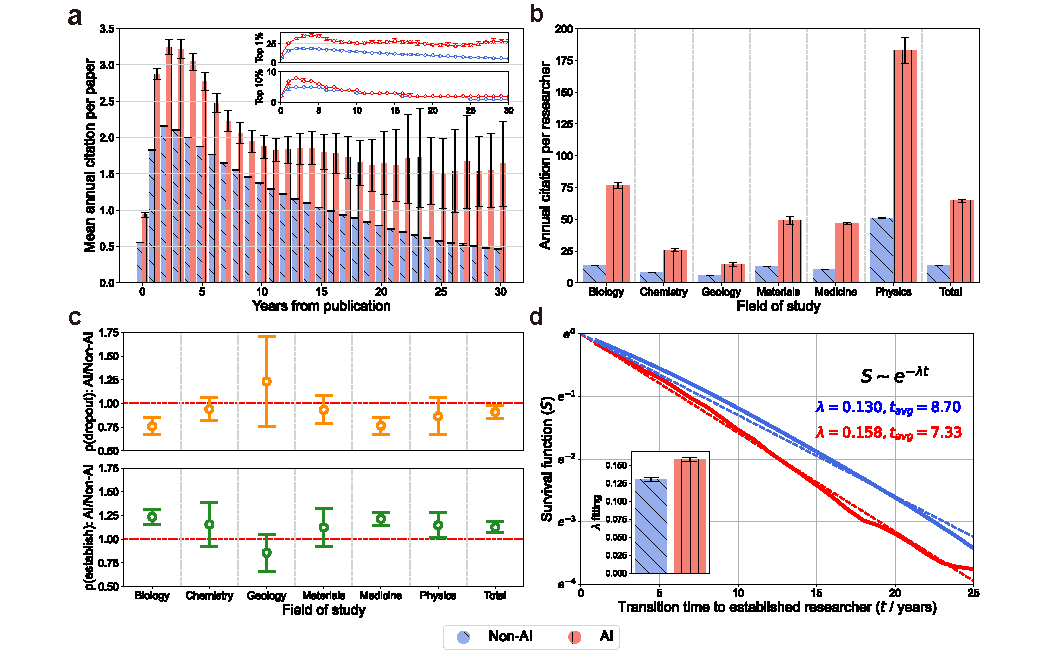
\includegraphics[width=\textwidth]{figure/2.pdf}
\caption{
\textbf{AI enlarges paper impact and enhances researcher careers.}
\textbf{(a)} Average (insets: top 1\% and 10\%) annual citations after publication of AI and non-AI papers ($n=27,405,011$), where AI papers attract more citations.
\textbf{(b)} Average annual citations for researchers adopting AI and their counterparts without AI ($p<0.001, n=5,377,346$), where researchers adopting AI garner 4.84 times more citations than their counterparts without AI.
\textbf{(c)} The probability of two role transitions between junior scientists adopting AI and their counterparts without AI ($n=46$ year observations for each field).
Junior scientists adopting AI have a higher probability of becoming established researchers and a lower probability of exiting academia compared with their counterparts without AI.
\textbf{(d)} Survival functions for the transition from junior to established researcher ($p<0.001, n=2,282,029$).
The survival function can be well-fit with exponential distributions, where junior scientists adopting AI become established earlier than their counterparts without AI.
For all panels, 99\% CIs are shown as error bars, with the insets of panel (a) centred at the 1\% and 10\% percentiles and other panels centred at the mean.
All statistical tests use a two-sided t-test.
}
\label{fig2}
\end{figure}

\subsection*{AI enhances individual scientists}
From statistics across 27,405,011 papers with intact reference records in the OpenAlex dataset, we note that from the publication date of each paper until decades later, annual citations to AI papers are 98.70\% higher than non-AI papers on average (Fig. 2a, $t\geq8.33$, $p<0.001$ and $df>10^3$ in t-test on any year).
In addition to higher annual average citations, the higher scientific impact of AI-augmented papers is also reflected by multiple alternative statistical indicators about top and bottom annual citation count (Supplementary Fig.~S8).
Also, AI papers published at different eras consistently receive more citations (Extended Data Fig. 3, $t\geq4.06$, $p<0.001$ and $df>10^3$ in t-test on any era).
Furthermore, we examine the distribution of AI-augmented papers across journals of varying Journal Citation Report (JCR) quantiles~\supercite{jcr} (Supplementary Fig.~S14).
We find that the proportion of AI papers in Q1 journals is 18.60\% higher than non-AI ones in all journals, and in Q2 journals, the AI proportion is 1.59\% higher, while Q3 and Q4 journals hold a relatively lower proportion of papers with AI ($\chi^2=3629.11$, $p<0.001$ and $df=3$ in $\chi^2$-test).
These results indicate a heterogeneous distribution of AI-augmented papers across journals, with a higher prevalence in high-impact journals.
Paralleled by the attention paid to AI papers, the impact of AI researchers also substantially increases.
On average, researchers adopting AI annually publish 3.02 times more papers ($t\geq47.18$, $p<0.001$ and $df>10^3$ in t-test on any discipline) and garner 4.84 times more citations ($t\geq30.32$, $p<0.001$ and $df>10^3$ in t-test on any discipline) compared with those not adopting AI, with consistency across disciplines and robustness for core researchers with multi-year continuous publication records~\supercite{ioannidis2014estimates} (Fig. 2b, Extended Data Fig. 4 and Supplementary Fig.~S17).
Furthermore, when controlling for and comparing scientists with similar early-career positions, the enhanced productivity and impact still hold (Supplementary Fig.~S16).
This suggests that, after accounting for potential selection-biases among researchers with different original achievements that may influence their choice of AI adoption, AI itself contributes to the observed advantages.

To identify the implications of AI adoption on scientist’s career development, we classify the scientists into “junior” and “established”, where junior scientists are defined as newcomers who have not yet led a research project, whereas established scientists refer to those who have led one or more research projects (Methods~M5 and Extended Data Fig. 5).
We extract 2,282,029 career trajectories of scientists from the dataset, each initially identified as a junior scientist (Methods~M6).
The results reveal that AI-augmented research is associated with reduced research team sizes, averaging 1.33 (19.29\%) fewer scientists ($t=20.47$, $p<0.001$ and $df>10^3$ in t-test, Extended Data Fig. 6).
Specifically, the average number of junior scientists decreased from 2.89 in non-AI teams to 1.99 (31.14\%) in AI teams ($t=19.02$, $p<0.001$ and $df>10^3$ in t-test), while the number of established scientists decreased from 4.01 to 3.58 (10.77\%) in AI teams ($t=20.82$, $p<0.001$ and $df>10^3$ in t-test).
This indicates that AI adoption primarily contributes to a reduction in the number of junior scientists in teams, while decrease in the number of established scientists is relatively moderate.
Given the decline in the number of junior scientists, we further calculate the probability of junior scientists becoming established scientists or leaving academia (Fig. 2c).
Across all studied disciplines, the probability for AI-adopted junior scientists to transition to established scientists is 45.00\%, 13.64\% higher than for their counterparts who do not adopt AI ($t\geq1.40$, $p<0.2$ and $df=90$ in t-test on 4 out of 6 disciplines).
This indicates that AI-adopted scientists are associated with increased opportunities to lead research projects and reduced risks of dropping out from academia, thereby experiencing accelerated career transitions from junior to established scientists.

To further quantify this effect, we measure the accelerated career development of junior scientists by employing a birth-death model~\supercite{kendall1960birth} and fitting the model parameter $\lambda$ with scientists’ career trajectories (Fig. 2d and Methods~M7).
We find that the anticipated transition time to becoming established scientists is 1.37 years shorter for AI-adopted junior scientists compared to their counterparts. The expectation of transition time is 7.33 years for junior scientists adopting AI ($R^2=0.995$) and 8.70 years for those without ($R^2=0.987$). 
This demonstrates how AI adoption affords junior scientists opportunities to lead research projects and become established earlier.
Further analysis reveals that this reduction in the transition time for AI-adopted junior scientists to become established ones is universal across examined disciplines (Extended Data Fig. 7).
Moreover, the established scientists involved in AI papers are, on average, 10.77\% younger than those in non-AI papers (Extended Data Fig. 6, $t\geq2.12$, $p<0.05$, and $df>10^3$ in t-test on most year).
Collectively, these findings suggest that AI research receives more attention from academia, and AI-adopting scientists are associated with higher scholarly productivity and impact.
In this way, they become established scientists with higher probability and at earlier ages, experiencing accelerated career development.


\begin{figure}[ht]
\centering
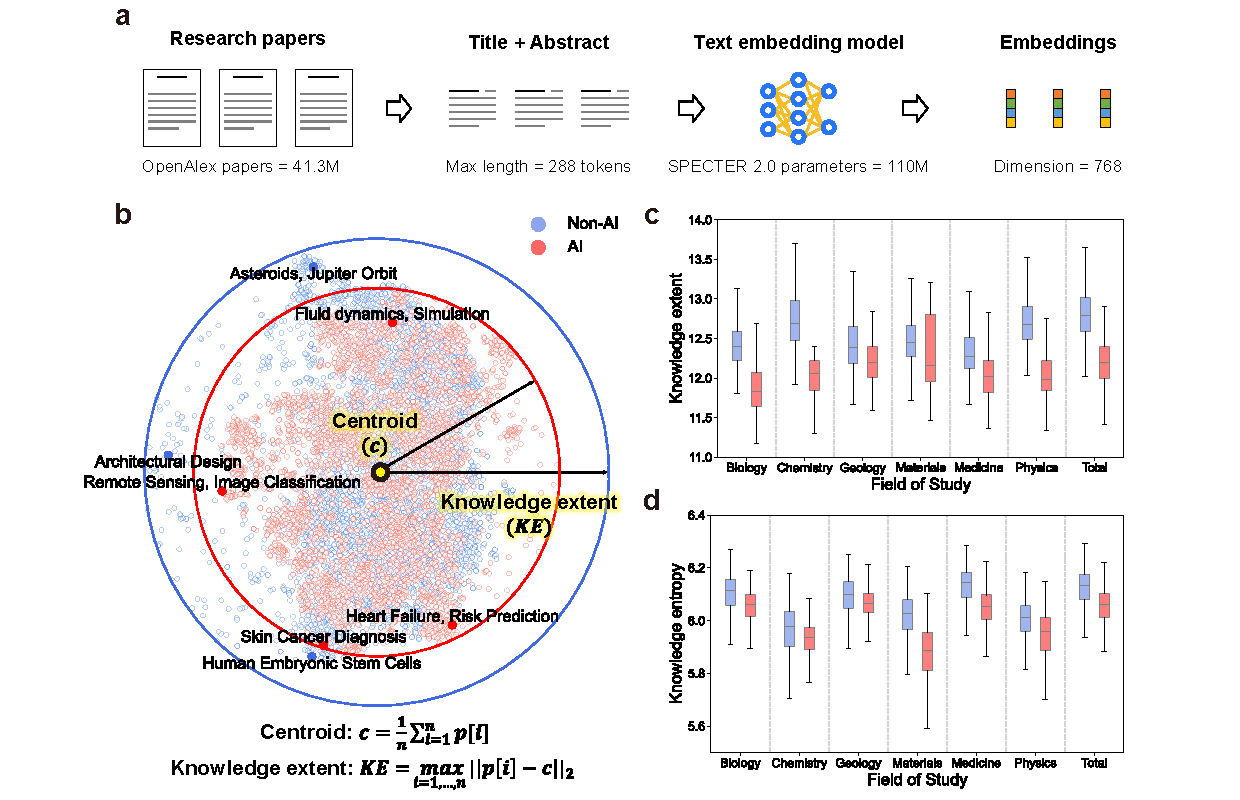
\includegraphics[width=\textwidth]{figure/3.pdf}
\caption{
\textbf{AI adoption is associated with a contraction in knowledge extent within and across scientific fields.}
\textbf{(a)} We embed research papers into a 768-dimensional vector space with a pre-trained text embedding model, then measure the knowledge extent of papers within that space.
\textbf{(b)} 
For visualization, we use the t-SNE algorithm to flatten the high-dimensional embeddings of a random batch of 10,000 papers, half of which are AI papers and half are non-AI papers, into a 2-D plot.
As shown by the solid arrows and circular boundaries, the knowledge extent of AI papers (calculated in the unflatted space) is smaller across the entirety of natural science, and AI papers are more clustered in knowledge space, indicating more concentration on specific problems.
\textbf{(c)} Knowledge extent of AI and non-AI papers in each field ($p<0.001, n=1,000$ samples in each field), where AI research focuses on a more contracted knowledge space.
\textbf{(d)} Knowledge entropy of AI and non-AI papers in each field ($p<0.001, n=1,000$ samples in each field), where AI research has a lower entropy.
For panels (c) and (d), boxplots are centred at the median and bounded at the first and third quartile (Q1 and Q3), with 1.5 times of the inter-quartile range (IQR) shown as whiskers from the box.
All statistical tests use a median-test.
}
\label{fig3}
\end{figure}

\subsection*{AI contracts science’s focus}
The accelerating use of AI in science and its impact on individual scientists raises questions about its influences across the entire scientific field.
To evaluate how AI collectively impacts the frontiers of scientific exploration, we design a measurement to characterize the breadth of scholarly attention represented by a collection of research papers.
We employ SPECTER 2.0, a specialized text embedding model pre-trained on a large scientific literature corpus and fine-tuned with citation information~\supercite{DBLP:conf/emnlp/SinghDCDF23}, to project research articles onto this 768-dimensional embedding space of science (Fig. 3a).

Within the high-dimensional embedding space, we design the measurement of knowledge extent (KE), which is the “diameter” of vector space covered by a sampled batch of papers, which allows us to compare the coverage of topical ground between AI and non-AI papers in each given domain~\supercite{fortunato2018science,milojevic2015quantifying} (Fig. 3b and Methods~M8).
Compared to conventional research, AI research is associated with a 4.63\% contracted median collective knowledge extent across science, which is consistent across all six disciplines (Fig. 3c and Extended Data Fig. 8, $\chi^2\geq84.05$, $p<0.001$ and $df=1$ in median-test on any discipline).
Moreover, when dividing these disciplines into more than two hundred sub-fields, the contraction of knowledge extent can be observed in more than 70\% of sub-fields (Extended Data Fig. 9).
When we compare the median entropy of knowledge distribution between AI and non-AI research in each domain (Fig. 3d), results demonstrate that the knowledge distribution of AI research has an lower entropy ($\chi^2\geq79.20$, $p<0.001$ and $df=1$ in median-test on any discipline), indicating an increasingly disproportionate focus on specific problems rather than across entire fields.

Generally, these results highlight an emerging conflict between individual and collective incentives to adopt AI in science, where scientists receive expanded personal reach and impact, but the knowledge extent of entire scientific fields tends to shrink and focus attention on a subset of topical areas.
According to analyses on possible factors that may influence the selectivity of AI adoption across different topics, we find that factors like inherent topicality, original impact, and funding priority, remain almost unrelated to the disproportionate AI adoption (Supplementary Fig.~S22-S24).
In contrast, data availability appears to be a major impacting factor, where areas with an abundance of data are increasingly and disproportionately amenable to AI research, contributing to the observed concentration within knowledge space (Supplementary Fig.~S25).


\begin{figure}[ht]
\centering
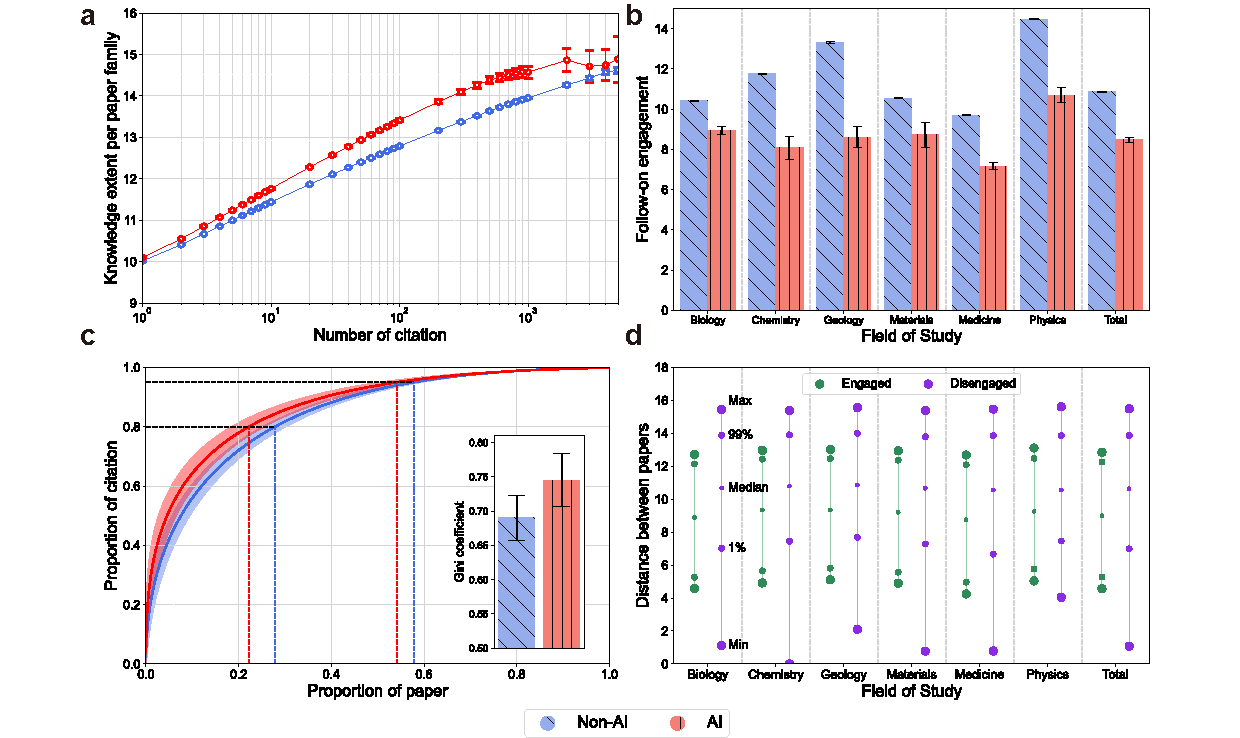
\includegraphics[width=\textwidth]{figure/4.pdf}
\caption{
\textbf{Reduced follow-on engagement and more overlapping works in AI research.}
\textbf{(a)} Knowledge extent of individual AI and non-AI paper families, i.e., an original paper and its cumulative citations ($n=27,405,011$), where the knowledge space of individual AI paper families is broader and grows faster.
\textbf{(b)} Engagement among papers that cite AI vs. non-AI papers ($p<0.001, n=23,342,516$), where there are fewer follow-on interactions among papers that cite the same original paper in AI research.
\textbf{(c)} Distribution of citations to AI vs. non-AI papers, where AI papers tend to concentrate more on a smaller number of top papers ($p<0.001, n=100$ sampled paper groups).
\textbf{(d)} Distribution of distances between paper pairs that cite the same prior research, with or without citing one another—engaged versus disengaged ($n=590,325,130$ sampled paper pairs).
Results show that for papers not engaged with each other, the median distance is larger, but the minimum distance is smaller, indicating a higher probability of overlapping in knowledge space.
For all panels, 99\% CIs are shown as error bars or error bands centred at the mean.
All statistical tests use a two-sided t-test.
}
\label{fig4}
\end{figure}


\subsection*{AI reduces scientific engagement}
In order to analyze mechanisms underlying the conflict between the growing influence of individual papers and researchers and the narrowing of domain knowledge within AI research, we examine the relationship between articles that cite AI and non-AI work.
We first examine the knowledge extent of “paper families”, i.e., a focal paper and its follow-on citations, which measures the size of the space covered by research derived from each original paper (Fig. 4a and Methods~M9).
Results show that the knowledge extent of AI papers’ citation families is on average 3.46\% \textit{more} expanded compared to non-AI papers’ ($t\geq1.91$, $p\leq0.1$ and $df>10^3$ in t-test on 30 out of 32 pairs of data).
Therefore, the contraction of knowledge space in AI research is not attributable to the narrowing of knowledge space that can be derived from each original research work.

To further investigate, we examine relationships between papers by measuring the degree of follow-on paper engagement, namely how frequently citations of the same original paper cite each other (Fig. 4b and Methods~M10).
Results demonstrate AI research spawns 22.00\% less follow-on engagement ($t\geq8.10$, $p<0.001$ and $df>10^3$ in t-test on any discipline), suggesting that AI papers tend to only concentrate on the original paper, rather than forming dense interactions among each other, which is the characteristic of emerging fields~\supercite{mcmahan2018ambiguity}.
This results in a star-like structure around specific popular research topics, rather than a network of emergent and interconnected research works.
Further evidence of this concentration is found in the Matthew effect~\supercite{merton1968matthew} among AI paper citations across different fields (Fig. 4c and Extended Data Fig. 10).
In AI research, a small number of superstar papers dominate the field, with 22.20\% of top papers receiving 80\% of the citations and the top 54.14\% receiving 95\% of citations. This unequal distribution leads to a GINI coefficient of 0.754 in citation patterns surrounding AI research, higher than 0.690 for non-AI papers ($t=27.86$, $p<0.001$ and $df=198$ in t-test), signaling a disparity in recognition.

To further analyze the impact of reduced follow-on engagement, we sample 590,325,130 pairs of papers, where each pair cites the same original work.
Among these, 51,723,984 pairs not only cite the same original work but also cite each other (engaged), while the remaining pairs do not cite each other (disengaged).
We examine distances between these pairs of papers within the 768-dimensional vector space (Fig. 4d) and find that median distance between paper pairs disengaged from one another tends to be 18.11\% larger than between paper pairs engaged with each other.
In contrast, the closest disengaged paper pairs are 76.51\% closer to one another than the closest paper pairs engaged with one another.
Taken together, a pair of disengaged papers commonly focus on less related topics and lie farther apart in the embedding space.
Occasionally, however, due to the lack of reciprocal engagement, it is possible that mutually-unaware papers lie very close to each other, which indicates more overlapping research.
These findings suggest that AI in science has become more concentrated around popular research topics that become “lonely crowds” with reduced interaction among papers, linking to more overlapping research and a contraction in knowledge extent and diversity across science.